\chapter{XÂY DỰNG ỨNG DỤNG DEMO VÀ HƯỚNG PHÁT TRIỂN}
\label{chap:chuong6}

\section{Mục tiêu và kiến trúc ứng dụng demo Streamlit}
\label{sec:muc-tieu-demo}

Theo quy định tại Mục 2.4 trong tài liệu hướng dẫn bài tập lớn của học phần FIT4013, các nhóm sinh viên xây dựng thành công ứng dụng giao diện người dùng (GUI/Demo) có tính hoàn thiện, hoạt động chính xác và có khả năng sử dụng thực tế sẽ được xem xét cộng từ \textbf{$0,5$ đến $1,0$ điểm thưởng}.

Để hiện thực hóa trọn vẹn mục tiêu này, Nhóm 13 đã thiết kế và phát triển ứng dụng web tương tác thời gian thực mang tên \textbf{“Hệ thống Phân loại Tin nhắn rác SMS”} bằng nền tảng \texttt{Streamlit} (mã nguồn tại \texttt{src/demo\_app.py}). Ứng dụng được thiết kế nhằm đáp ứng ba mục tiêu trọng tâm:
\begin{enumerate}
    \item \textbf{Tính thực tế và thân thiện (Usability):} Cung cấp giao diện trực quan cho phép người dùng hoặc giảng viên chấm thi có thể nhập bất kỳ tin nhắn văn bản nào hoặc lựa chọn các kịch bản mẫu để kiểm chứng khả năng phân loại tức thời.
    \item \textbf{Tính minh bạch và so sánh đa mô hình (Multi-model Transparency):} Không chỉ hiển thị kết quả của mô hình tốt nhất, ứng dụng tích hợp song song cả ba mô hình tối ưu đã nghiên cứu (Multinomial Naive Bayes, K-NN và Cây quyết định), cho phép đối chiếu trực tiếp sự đồng thuận hoặc bất đồng giữa các trường phái thuật toán trên cùng một văn bản.
    \item \textbf{Tính giải thích được (Explainable AI --- XAI):} Tích hợp cơ chế "Mở hộp đen" (Open the Black Box), hiển thị rõ ràng chuỗi ký tự sau khi qua bộ tiền xử lý và bảng phân rã đóng góp xác suất (Log-Odds Attribution) của từng từ vựng, giúp người dùng hiểu chính xác *vì sao* mô hình lại đưa ra quyết định đó.
\end{enumerate}

Về kiến trúc phần mềm, ứng dụng tuân thủ mô hình phân tầng gọn nhẹ:
\begin{itemize}
    \item \textbf{Tầng dữ liệu và mô hình (Backend Engine):} Hàm \texttt{train\_models()} nạp dữ liệu sạch từ \texttt{src/common.py}, khởi tạo 3 đường ống \texttt{Pipeline} với cấu hình tối ưu đã được thẩm định chéo ở Chương 4, và huấn luyện trên 80\% tập Train. Hàm được gắn bộ trang trí \texttt{@st.cache\_resource} của Streamlit: quá trình huấn luyện chỉ diễn ra một lần duy nhất trong vài giây khi khởi động server, toàn bộ các lượt dự đoán sau đó được truy xuất tức thời từ bộ nhớ RAM với độ trễ xấp xỉ 0 mili-giây.
    \item \textbf{Tầng giao diện người dùng (Frontend UI):} Xây dựng hoàn toàn bằng ngôn ngữ Python thông qua các widget phản ứng (Reactive Widgets) của Streamlit, hỗ trợ tự động mở trình duyệt web tại địa chỉ cục bộ \texttt{http://localhost:8501}.
\end{itemize}

\noindent\textbf{*Cấu trúc thư mục:}
\begin{figure}[H]
    \centering
    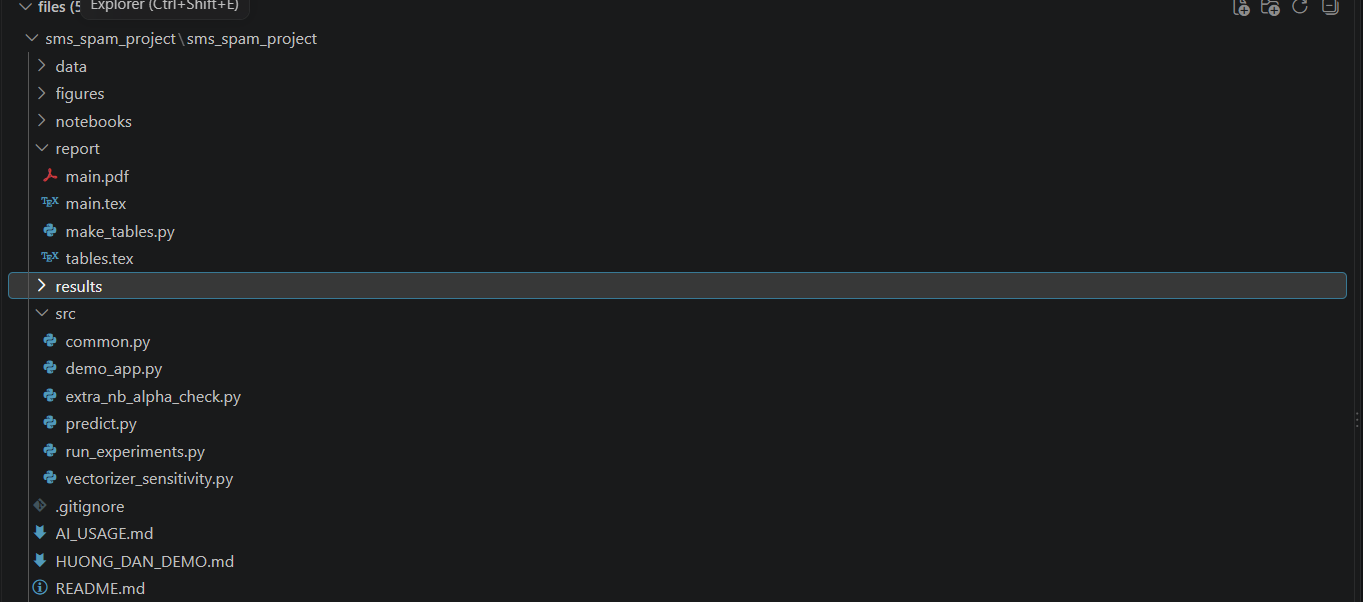
\includegraphics[width=0.85\textwidth]{images/demo_tree_structure.png}
    \caption{Cấu trúc thư mục mã nguồn và các module thành phần của dự án}
    \label{fig:demo-tree-structure}
\end{figure}

\noindent\textbf{*Toàn cảnh giao diện:}
\begin{figure}[H]
    \centering
    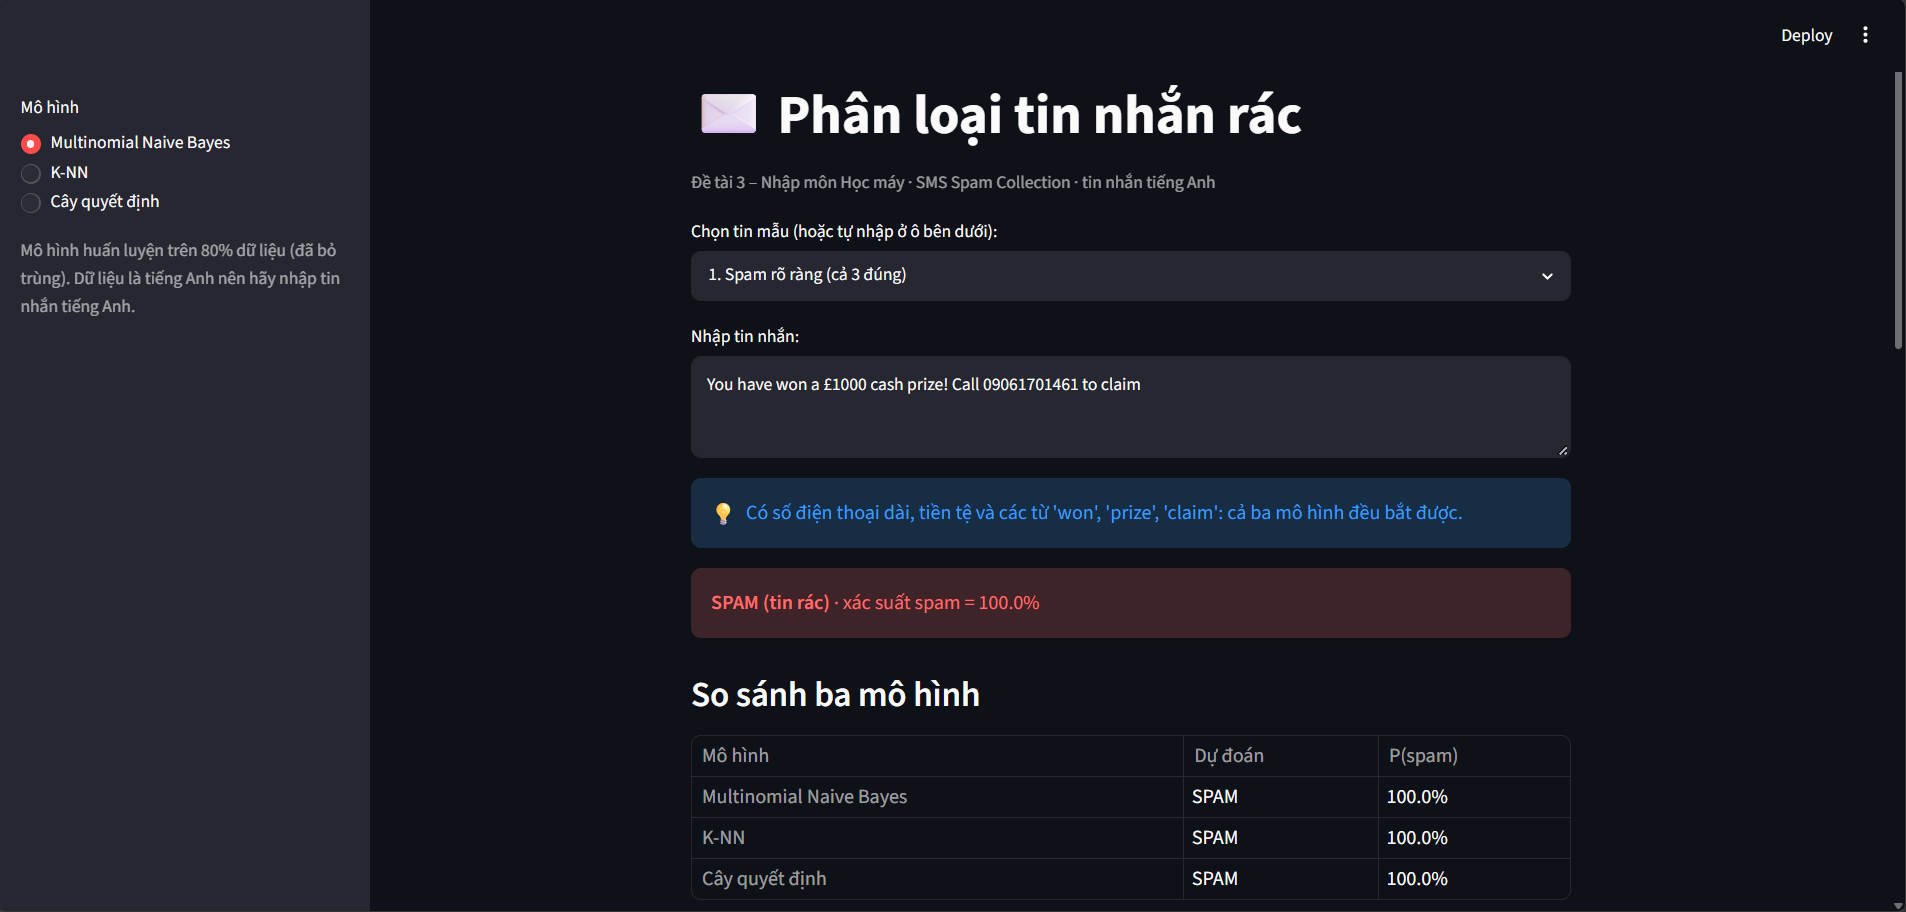
\includegraphics[width=0.95\textwidth]{images/demo_overview.png}
    \caption{Toàn cảnh giao diện ứng dụng web tương tác phân loại tin nhắn rác Streamlit}
    \label{fig:demo-overview}
\end{figure}

\section{Chi tiết thiết kế giao diện và trải nghiệm người dùng}
\label{sec:thiet-ke-giao-dien}

Giao diện ứng dụng được bố cục khoa học, hiện đại gồm ba khu vực chức năng chính:

\subsection{Thanh điều khiển bên (Sidebar Panel)}

\begin{figure}[H]
    \centering
    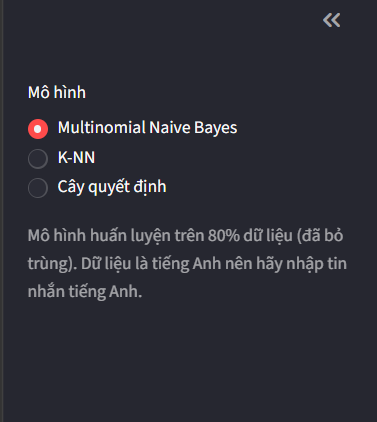
\includegraphics[width=0.55\textwidth]{images/demo_sidebar.png}
    \caption{Giao diện thanh điều khiển bên (Sidebar) cho phép chuyển đổi linh hoạt giữa 3 mô hình}
    \label{fig:demo-sidebar}
\end{figure}

Nằm ở cột bên trái màn hình, cung cấp:
\begin{itemize}
    \item Nút radio cho phép người dùng lựa chọn mô hình phân loại trung tâm:
    \begin{itemize}
        \item Multinomial Naive Bayes (Mô hình tối ưu tổng thể);
        \item K-Nearest Neighbors (Mô hình dựa trên láng giềng Cosine);
        \item Cây quyết định (Mô hình dựa trên luật cứng).
    \end{itemize}
    \item Phần chú thích (Caption) hướng dẫn người dùng: mô hình được huấn luyện trên ngữ liệu tiếng Anh, do đó các văn bản kiểm thử cần được soạn thảo bằng tiếng Anh để đảm bảo tính chuẩn xác.
\end{itemize}

\subsection{Khu vực nhập liệu và hiển thị kết quả trung tâm}

\noindent\textbf{*Giao diện chính:}
\begin{figure}[H]
    \centering
    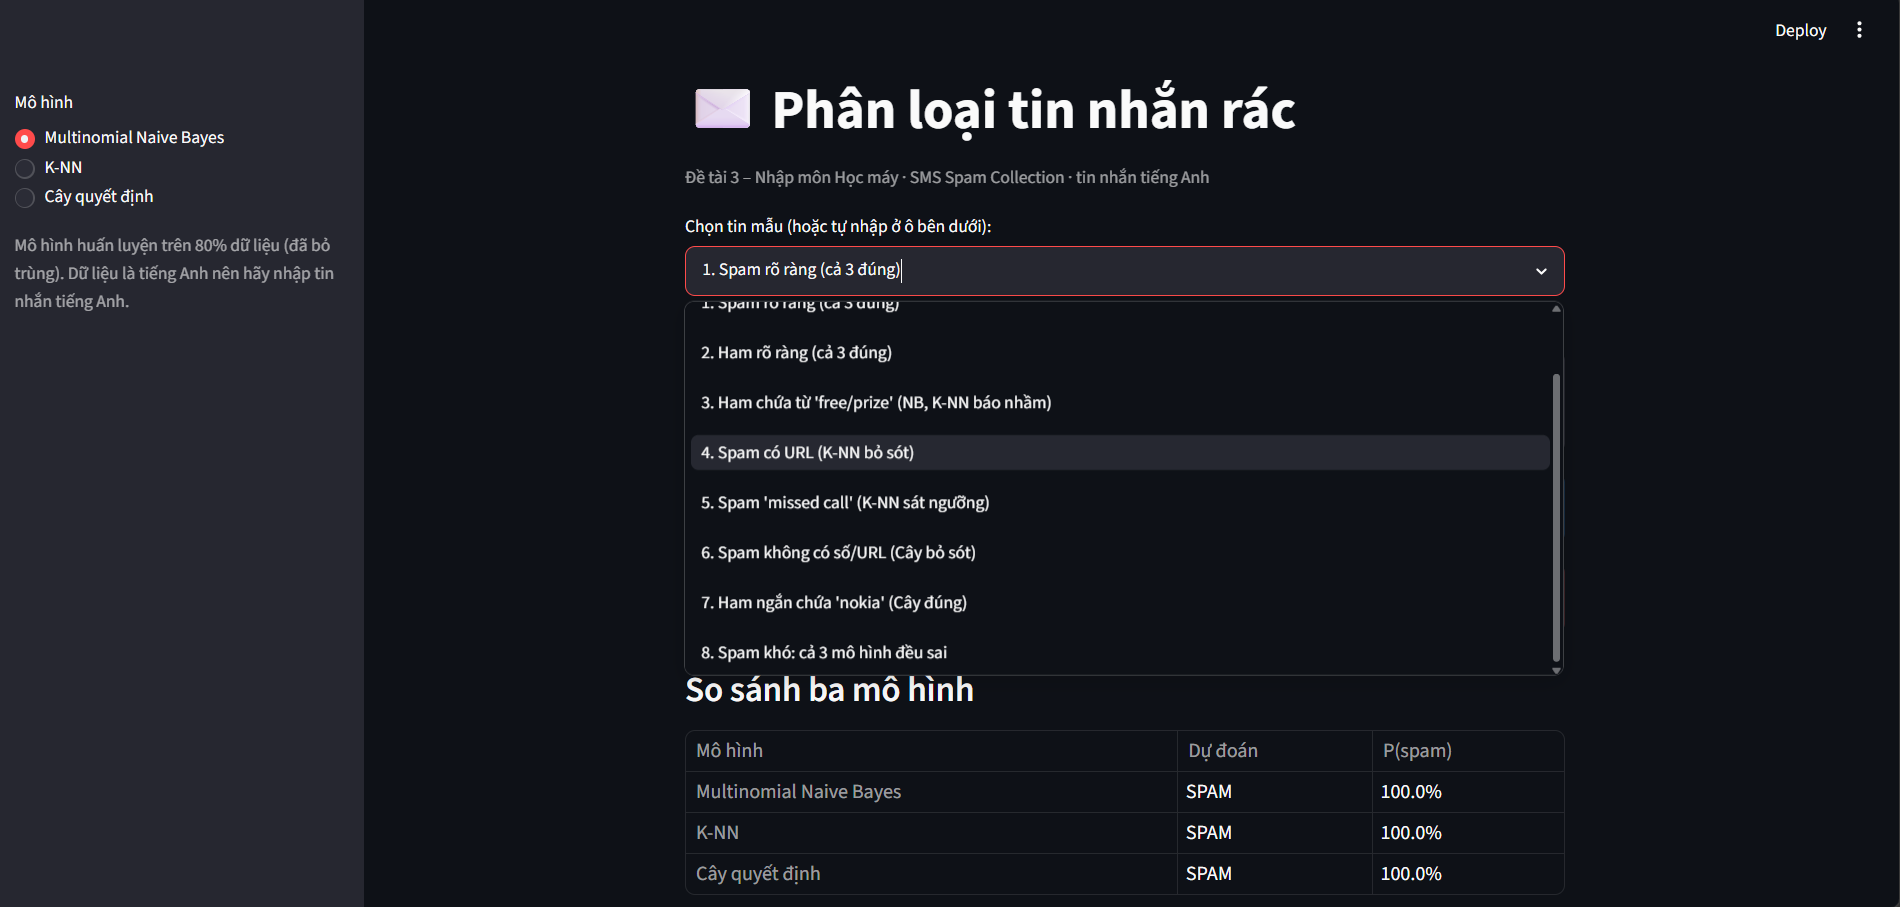
\includegraphics[width=0.95\textwidth]{images/demo_main_input.png}
    \caption{Khu vực trung tâm với hộp chọn kịch bản mẫu và khung soạn thảo văn bản}
    \label{fig:demo-main-input}
\end{figure}

Nằm ở khung hình chính, bao gồm:
\begin{itemize}
    \item Hộp danh sách thả xuống (\texttt{st.selectbox}) chứa \textbf{8 tin nhắn mẫu kinh điển} được thiết kế sẵn. Khi người dùng bấm chọn một tin mẫu, nội dung tin nhắn sẽ tự động được điền vào khung soạn thảo văn bản bên dưới, kèm theo một hộp thông tin gợi ý phân tích (Info Callout) giải thích trước hiện tượng kỹ thuật sẽ diễn ra.
    \item Ô nhập văn bản đa dòng (\texttt{st.text\_area}): Cho phép người dùng tự do gõ hoặc dán bất kỳ tin nhắn nào từ clipboard.
    \item Khối thông báo trạng thái phân loại:
    \begin{itemize}
        \item Nếu dự đoán là tin rác: Hiển thị hộp cảnh báo màu đỏ rực rỡ (\texttt{st.error}) với dòng chữ in đậm: \textbf{“SPAM (tin rác) · xác suất spam = XX.X\%”}.
        \item Nếu dự đoán là tin hợp lệ: Hiển thị hộp thông báo màu xanh lá cây an toàn (\texttt{st.success}) với dòng chữ: \textbf{“HAM (tin hợp lệ) · xác suất spam = XX.X\%”}.
    \end{itemize}
    \item Bảng đối sánh song song ba mô hình (\texttt{st.table}): Trình bày bảng so sánh trực quan gồm ba cột: Tên mô hình, Nhãn dự đoán (SPAM/HAM) và Xác suất spam tính theo tỷ lệ phần trăm $P(\text{spam})$.
\end{itemize}

\noindent\textbf{*Minh chứng kết quả phân loại:}

\noindent\textbf{SPAM:}
\begin{figure}[H]
    \centering
    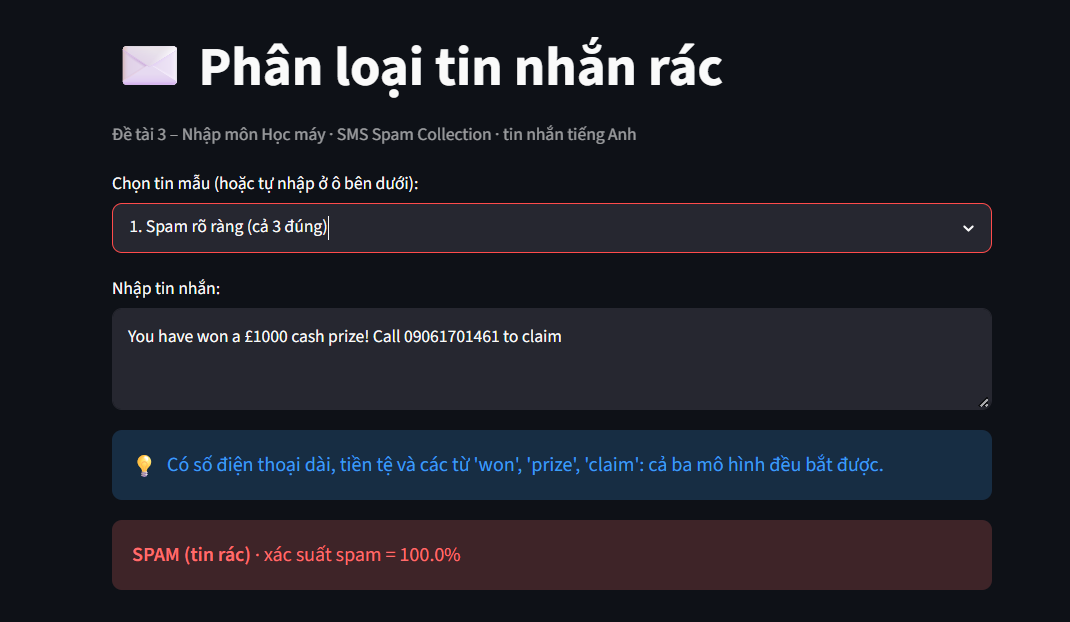
\includegraphics[width=0.92\textwidth]{images/demo_result_spam.png}
    \caption{Hộp cảnh báo màu đỏ rực rỡ khi mô hình phát hiện tin nhắn SPAM}
    \label{fig:demo-result-spam}
\end{figure}

\noindent\textbf{HAM:}
\begin{figure}[H]
    \centering
    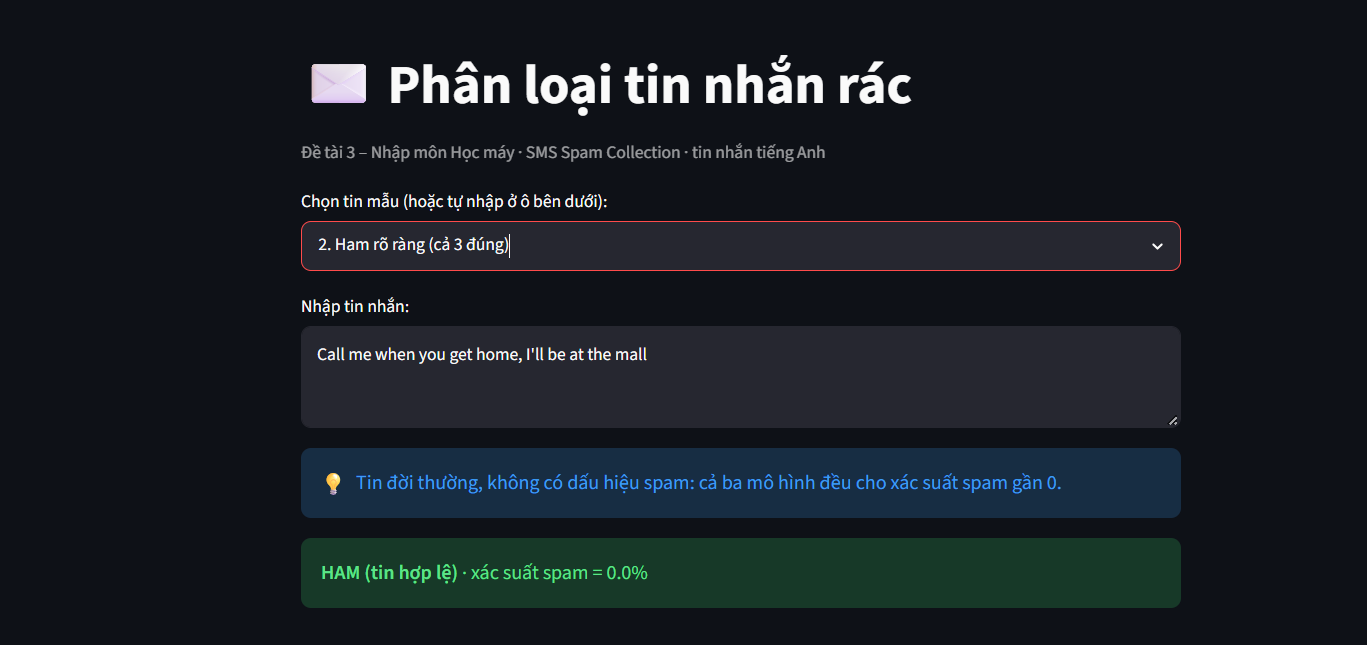
\includegraphics[width=0.92\textwidth]{images/demo_result_ham.png}
    \caption{Hộp thông báo màu xanh lá cây an toàn khi mô hình xác định tin nhắn hợp lệ HAM}
    \label{fig:demo-result-ham}
\end{figure}

\noindent\textbf{*Bảng so sánh 3 mô hình:}
\begin{figure}[H]
    \centering
    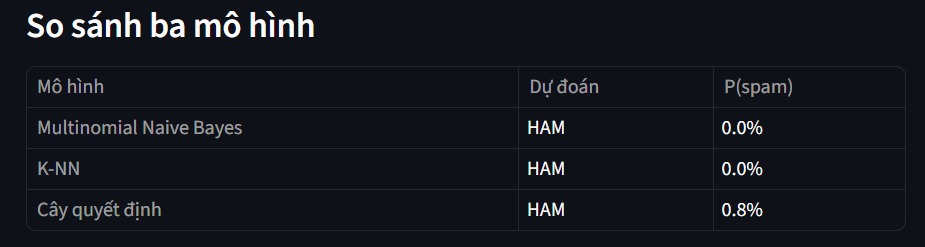
\includegraphics[width=0.85\textwidth]{images/demo_model_comparison.png}
    \caption{Bảng so sánh kết quả dự đoán và xác suất spam của cả ba mô hình trên cùng một tin nhắn}
    \label{fig:demo-model-comparison}
\end{figure}

\subsection{Khối giải thích cơ chế mô hình (Model Explainability Panel)}
Nằm trong một khối đóng mở linh hoạt (\texttt{st.expander}) với tiêu đề *“Mô hình nhìn thấy gì? (tiền xử lý và từ ảnh hưởng)”*:
\begin{enumerate}
    \item \textbf{Hiển thị văn bản sau chuẩn hóa:} Khối mã nguồn hiển thị chuỗi văn bản sau khi đã đi qua hàm \texttt{normalize\_text}. Người dùng có thể quan sát trực tiếp cách các số điện thoại dài bị biến thành \texttt{longnumtoken}, đường dẫn web thành \texttt{urltoken} và ký hiệu tiền tệ thành \texttt{currtoken}.
    \item \textbf{Bảng phân rã đóng góp từ vựng (Feature Contribution Table):}
    Khi mô hình được chọn là Multinomial Naive Bayes, hệ thống trích xuất toàn bộ các từ trong tin nhắn có mặt trong từ điển của mô hình, tính toán mức độ đóng góp theo công thức:
    \begin{equation}
    \text{Contribution}(w_i) = \text{count}(w_i) \times \left[ \ln \hat{P}(w_i | \text{spam}) - \ln \hat{P}(w_i | \text{ham}) \right]
    \end{equation}
    và hiển thị dưới dạng bảng dữ liệu có thể cuộn, sắp xếp từ có giá trị đóng góp dương lớn nhất (kéo mạnh về phía SPAM) đến các từ có giá trị âm lớn nhất (kéo mạnh về phía HAM). Đây là tính năng minh chứng rõ nét cho việc sinh viên làm chủ trọn vẹn bản chất toán học của thuật toán.
\end{enumerate}

\begin{figure}[H]
    \centering
    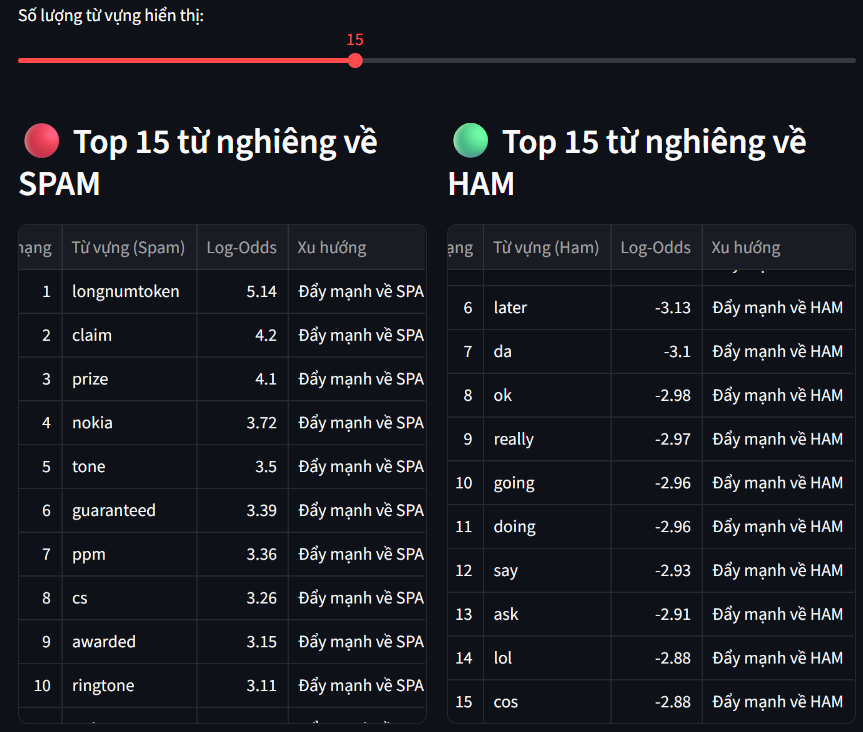
\includegraphics[width=0.95\textwidth]{images/demo_explainability.png}
    \caption{Khối giải thích "Mở hộp đen" với chuỗi tiền xử lý và bảng phân rã đóng góp xác suất Log-Odds}
    \label{fig:demo-explainability}
\end{figure}

\section{Bộ 8 kịch bản kiểm thử mẫu (Demonstration Test Cases)}
\label{sec:8-kich-ban-mau}

Để phục vụ công tác báo cáo và bảo vệ đồ án trước Hội đồng chấm thi một cách thuyết phục nhất, nhóm đã biên soạn một kịch bản trình diễn chuẩn xác gồm 8 tình huống kiểm thử (được lưu trữ tại \texttt{HUONG\_DAN\_DEMO.md}). Các tình huống này được lựa chọn có chủ đích nhằm làm nổi bật cả ưu điểm lẫn các ranh giới bất đồng giữa ba trường phái học máy.

\subsection{Chi tiết 8 kịch bản kiểm thử mẫu}
\begin{enumerate}
    \item \textbf{Tin mẫu 1 --- Spam rõ ràng đầy đủ dấu hiệu (Cả 3 mô hình cùng đúng):}
    \begin{figure}[H]
        \centering
        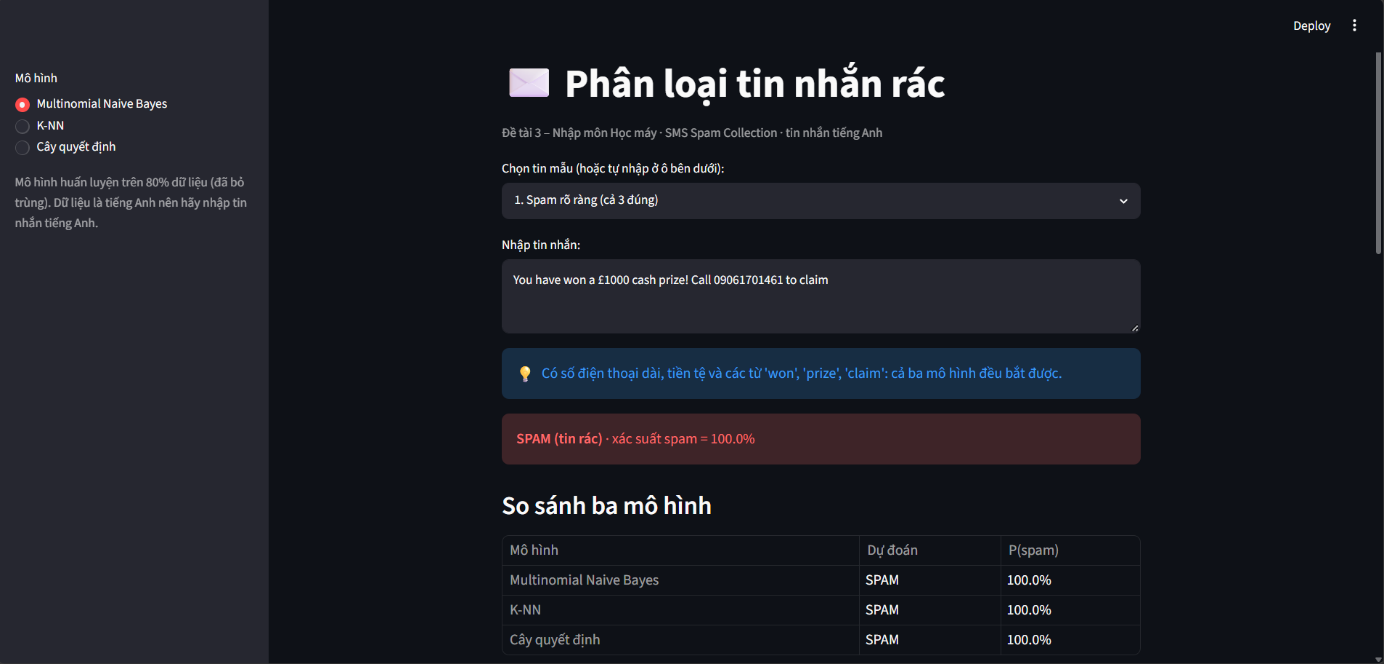
\includegraphics[width=0.92\textwidth]{images/demo_case1.png}
        \caption{Minh chứng thực nghiệm Tin mẫu 1 trên giao diện Demo}
        \label{fig:demo-case1}
    \end{figure}
    \begin{itemize}
        \item \textit{Nội dung:} \texttt{“You have won a £1000 cash prize! Call 09061701461 to claim”}
        \item \textit{Phân tích kỹ thuật:} Tin nhắn chứa đồng thời ký hiệu tiền tệ (£ $\rightarrow$ \texttt{currtoken}), chuỗi số dài (\texttt{longnumtoken}) và các từ khóa đặc trưng (\texttt{won}, \texttt{prize}, \texttt{claim}). Cả ba mô hình đều dự đoán SPAM với xác suất tuyệt đối $100\%$.
    \end{itemize}
    
    \item \textbf{Tin mẫu 2 --- Ham rõ ràng thường nhật (Cả 3 mô hình cùng đúng):}
    \begin{figure}[H]
        \centering
        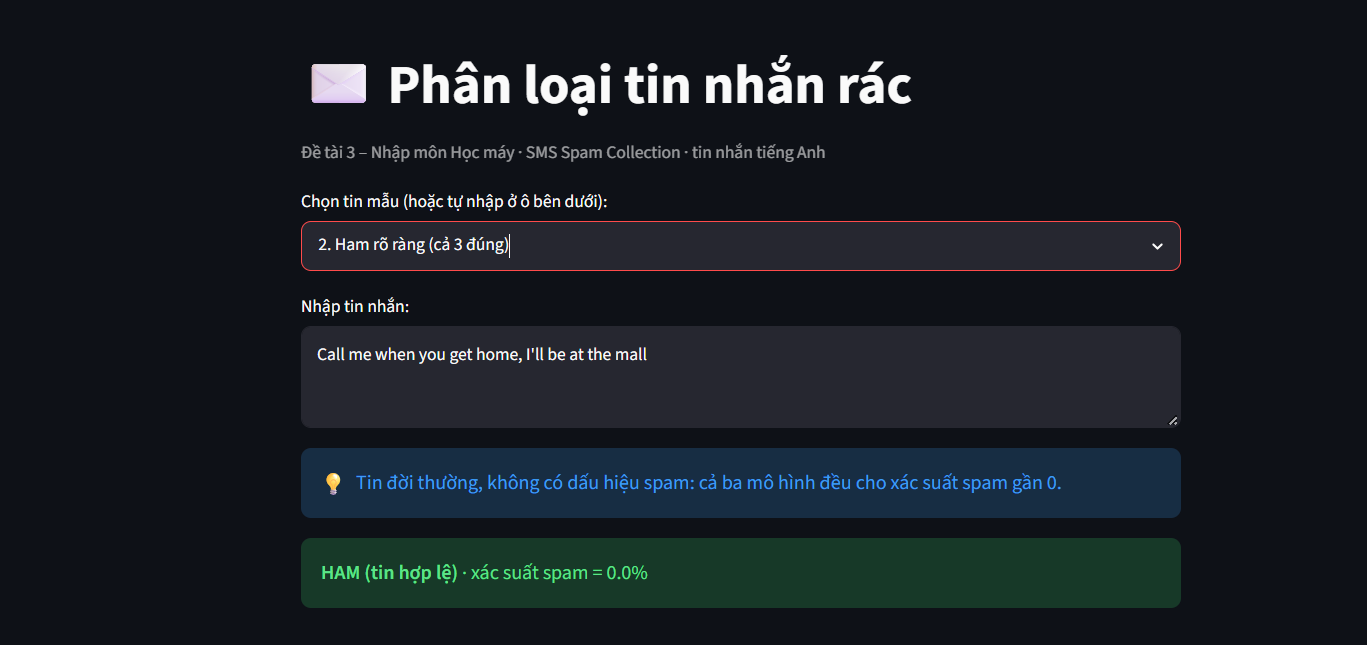
\includegraphics[width=0.92\textwidth]{images/demo_result_ham.png}
        \caption{Minh chứng thực nghiệm Tin mẫu 2 trên giao diện Demo}
        \label{fig:demo-case2}
    \end{figure}
    \begin{itemize}
        \item \textit{Nội dung:} \texttt{“Call me when you get home, I'll be at the mall”}
        \item \textit{Phân tích kỹ thuật:} Tin nhắn giao tiếp gia đình, chứa các từ đời thường (\texttt{call}, \texttt{home}, \texttt{mall}). Cả ba mô hình đều dự đoán HAM với xác suất spam gần bằng $0\%$.
    \end{itemize}
    
    \item \textbf{Tin mẫu 3 --- Ham chứa từ khóa nhạy cảm (Naive Bayes và K-NN báo nhầm; Cây quyết định đúng):}
    \begin{figure}[H]
        \centering
        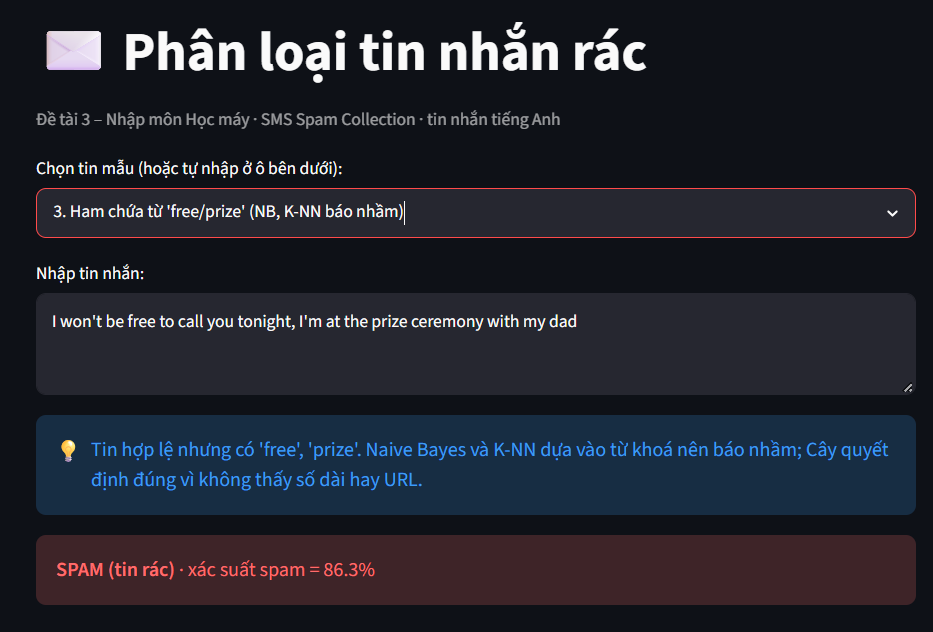
\includegraphics[width=0.92\textwidth]{images/demo_case3.png}
        \caption{Minh chứng thực nghiệm Tin mẫu 3 trên giao diện Demo}
        \label{fig:demo-case3}
    \end{figure}
    \begin{itemize}
        \item \textit{Nội dung:} \texttt{“I won't be free to call you tonight, I'm at the prize ceremony with my dad”}
        \item \textit{Phân tích kỹ thuật:} Tin nhắn hoàn toàn hợp lệ của sinh viên nhắn cho người thân, nhưng có chứa hai từ ngữ nhạy cảm thường thấy trong tin nhắn rác là \texttt{free} và \texttt{prize}. Do Naive Bayes cộng dồn điểm log-odds của từng từ độc lập và K-NN tìm kiếm láng giềng dựa trên trùng lặp từ khóa, cả hai mô hình này đều phát chuông báo động nhầm (Dương tính giả FP). Ngược lại, Cây quyết định dự đoán chính xác là HAM vì cây kiểm tra quy tắc cấu trúc: tin nhắn không chứa số điện thoại dài (\texttt{longnumtoken}) hay đường dẫn web (\texttt{urltoken}).
    \end{itemize}
    
    \item \textbf{Tin mẫu 4 --- Spam chứa liên kết URL (Cây quyết định đúng; K-NN bỏ sót):}
    \begin{figure}[H]
        \centering
        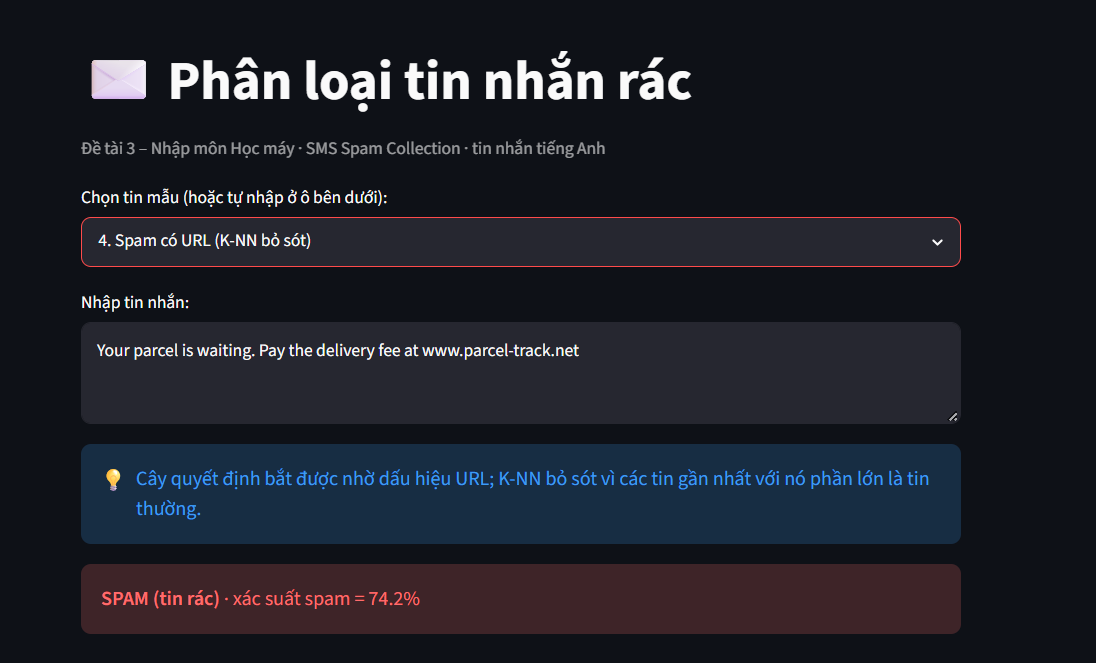
\includegraphics[width=0.92\textwidth]{images/demo_case4.png}
        \caption{Minh chứng thực nghiệm Tin mẫu 4 trên giao diện Demo}
        \label{fig:demo-case4}
    \end{figure}
    \begin{itemize}
        \item \textit{Nội dung:} \texttt{“Your parcel is waiting. Pay the delivery fee at www.parcel-track.net”}
        \item \textit{Phân tích kỹ thuật:} Tin nhắn lừa đảo mạo danh bưu điện phát tán đường dẫn web. Cây quyết định bắt gọn nhờ nhánh kiểm tra \texttt{urltoken}. Tuy nhiên, K-NN bỏ sót (Âm tính giả FN) do các từ đời thường như *“parcel”*, *“waiting”*, *“delivery”* khiến tin nhắn này nằm gần các mẫu tin nhắn hợp lệ trong không gian biểu diễn.
    \end{itemize}
    
    \item \textbf{Tin mẫu 5 --- Spam cuộc gọi nhỡ (Cây quyết định và Naive Bayes đúng; K-NN sát ngưỡng):}
    \begin{figure}[H]
        \centering
        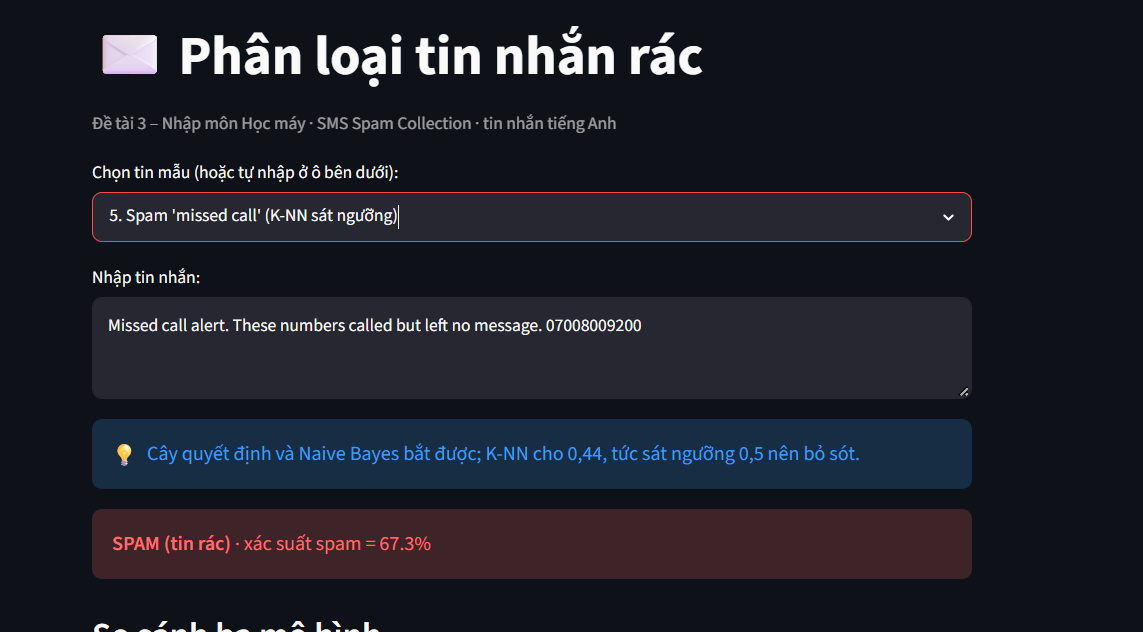
\includegraphics[width=0.92\textwidth]{images/demo_case5.png}
        \caption{Minh chứng thực nghiệm Tin mẫu 5 trên giao diện Demo}
        \label{fig:demo-case5}
    \end{figure}
    \begin{itemize}
        \item \textit{Nội dung:} \texttt{“Missed call alert. These numbers called but left no message. 07008009200”}
        \item \textit{Phân tích kỹ thuật:} Cây quyết định và Naive Bayes bắt chính xác nhờ chuỗi số dài $11$ chữ số (\texttt{longnumtoken}). K-NN tính toán xác suất spam đạt $44\%$, nằm sát ngưỡng phân định $50\%$ nhưng vẫn bị phân loại sót thành ham do biểu quyết đa số.
    \end{itemize}
    
    \item \textbf{Tin mẫu 6 --- Spam không chứa số dài hay URL (Naive Bayes và K-NN đúng; Cây quyết định bỏ sót):}
    \begin{figure}[H]
        \centering
        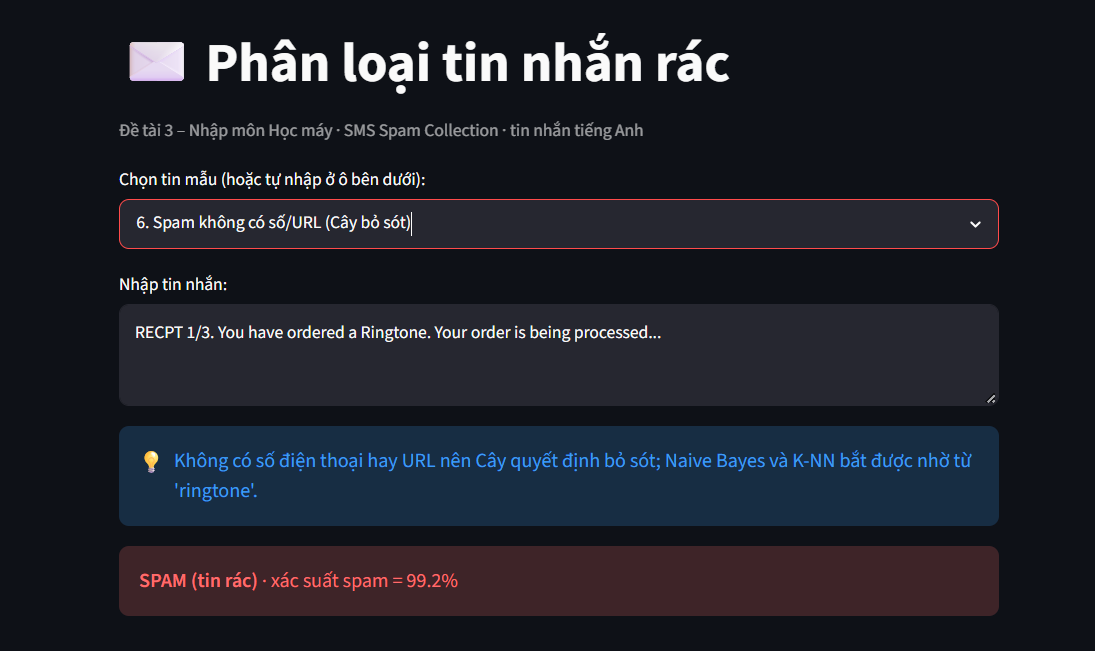
\includegraphics[width=0.92\textwidth]{images/demo_case6.png}
        \caption{Minh chứng thực nghiệm Tin mẫu 6 trên giao diện Demo}
        \label{fig:demo-case6}
    \end{figure}
    \begin{itemize}
        \item \textit{Nội dung:} \texttt{“RECPT 1/3. You have ordered a Ringtone. Your order is being processed...”}
        \item \textit{Phân tích kỹ thuật:} Tin nhắn spam dịch vụ nhạc chuông nhưng không để lại số hotline hay website liên hệ. Cây quyết định bị bỏ sót (FN) do không thỏa mãn luật kiểm tra nút gốc. Ngược lại, Naive Bayes và K-NN nhận diện thành công nhờ trọng số từ vựng tiếp thị mạnh của từ \texttt{ringtone} và \texttt{ordered}.
    \end{itemize}
    
    \item \textbf{Tin mẫu 7 --- Ham ngắn chứa từ thương hiệu (Naive Bayes và K-NN nhầm; Cây quyết định đúng):}
    \begin{figure}[H]
        \centering
        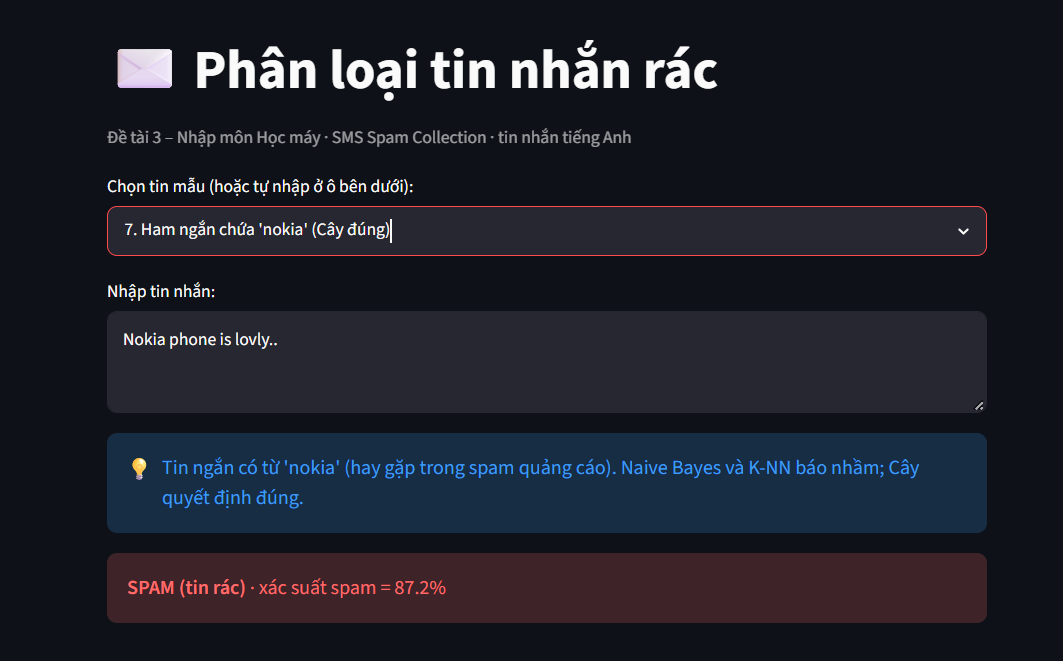
\includegraphics[width=0.92\textwidth]{images/demo_case7.png}
        \caption{Minh chứng thực nghiệm Tin mẫu 7 trên giao diện Demo}
        \label{fig:demo-case7}
    \end{figure}
    \begin{itemize}
        \item \textit{Nội dung:} \texttt{“Nokia phone is lovly..”}
        \item \textit{Phân tích kỹ thuật:} Đây chính là ca Dương tính giả (FP) kinh điển đã mổ xẻ tại Chương 5. Naive Bayes và K-NN bị từ \texttt{nokia} đánh lừa; Cây quyết định giữ vững sự kiên định nhờ không có số dài.
    \end{itemize}
    
    \item \textbf{Tin mẫu 8 --- Spam tinh vi dạng câu đố truyền thông (Cả 3 mô hình cùng sai):}
    \begin{figure}[H]
        \centering
        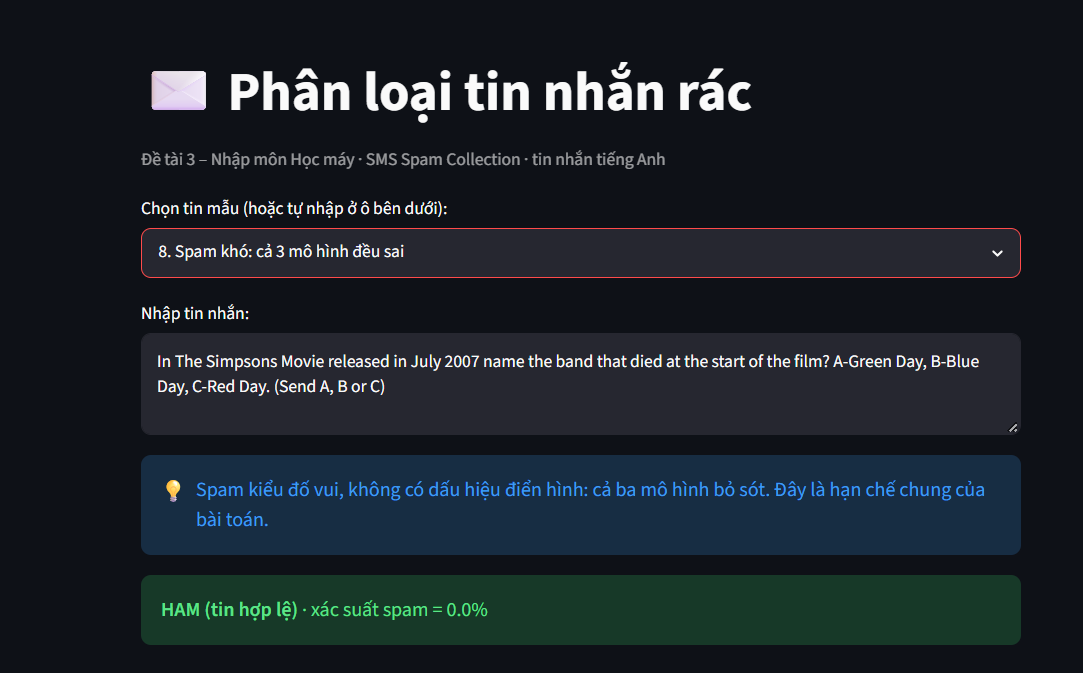
\includegraphics[width=0.92\textwidth]{images/demo_case8.png}
        \caption{Minh chứng thực nghiệm Tin mẫu 8 trên giao diện Demo}
        \label{fig:demo-case8}
    \end{figure}
    \begin{itemize}
        \item \textit{Nội dung:} \texttt{“In The Simpsons Movie released in July 2007 name the band that died at the start of the film? A-Green Day, B-Blue Day, C-Red Day. (Send A, B or C)”}
        \item \textit{Phân tích kỹ thuật:} Ca Âm tính giả (FN) chung của cả ba mô hình. Tin nhắn hoàn toàn thiếu vắng các từ khóa tiếp thị và tín hiệu cấu trúc, minh chứng cho giới hạn tự nhiên của các mô hình học máy dựa trên túi từ BoW và TF-IDF.
    \end{itemize}
\end{enumerate}

\subsection{Kịch bản trình diễn 5 phút trước Hội đồng bảo vệ}
Nhóm đã đúc kết quy trình thuyết trình sản phẩm trực quan gồm 5 bước chặt chẽ:
\begin{itemize}
    \item \textbf{Phút 0:00 -- 0:30:} Mở giao diện Streamlit tại \texttt{localhost:8501}, giới thiệu tổng quan đề tài, quy mô dữ liệu và bài toán phân loại nhị phân mất cân bằng.
    \item \textbf{Phút 0:30 -- 1:15:} Giới thiệu bố cục giao diện, thanh chọn mô hình và bảng đối sánh kết quả ba mô hình song song.
    \item \textbf{Phút 1:15 -- 2:00:} Trình diễn Tin mẫu 1 (Spam rõ) và Tin mẫu 2 (Ham rõ), giải thích rằng với 98,2\% tin nhắn thông thường cả 3 mô hình đều đồng thuận tuyệt đối.
    \item \textbf{Phút 2:00 -- 4:00:} Trình diễn các trường hợp bất đồng kỹ thuật sâu sắc: Tin mẫu 3 (giải thích vì sao Cây quyết định thông minh hơn Naive Bayes khi gặp từ \texttt{free}/\texttt{prize}), Tin mẫu 6 (giải thích vì sao Naive Bayes bắt được \texttt{ringtone} còn Cây bị mù). Mở bảng Log-Odds Attribution để chứng minh cơ chế tính điểm toán học.
    \item \textbf{Phút 4:00 -- 5:00:} Trình diễn Tin mẫu 8 (thừa nhận trung thực hạn chế của mô hình trước spam câu đố) và kết luận về việc lựa chọn mô hình Naive Bayes kết hợp điều chỉnh ngưỡng quyết định trong thực tiễn.
\end{itemize}

\section{Công cụ dòng lệnh CLI (\texttt{src/predict.py})}
\label{sec:cli-predict}

Bên cạnh giao diện web đồ họa Streamlit, nhóm đã phát triển công cụ dòng lệnh độc lập \texttt{src/predict.py} nhằm phục vụ mục đích tự động hóa, kiểm thử hàng loạt (Batch testing) hoặc tích hợp mô hình vào các đường ống xử lý ngầm (Backend daemons/Cron jobs).

\subsection{Phương thức vận hành}
Chương trình tự động nạp mô hình tối ưu đã lưu tại \texttt{results/best\_model.joblib} và vận hành linh hoạt theo hai chế độ:
\begin{enumerate}
    \item \textbf{Chế độ đối số dòng lệnh (Command-line arguments):}
    Truyền trực tiếp một hoặc nhiều chuỗi tin nhắn văn bản vào đối số thực thi:
    
    \begin{figure}[H]
        \centering
        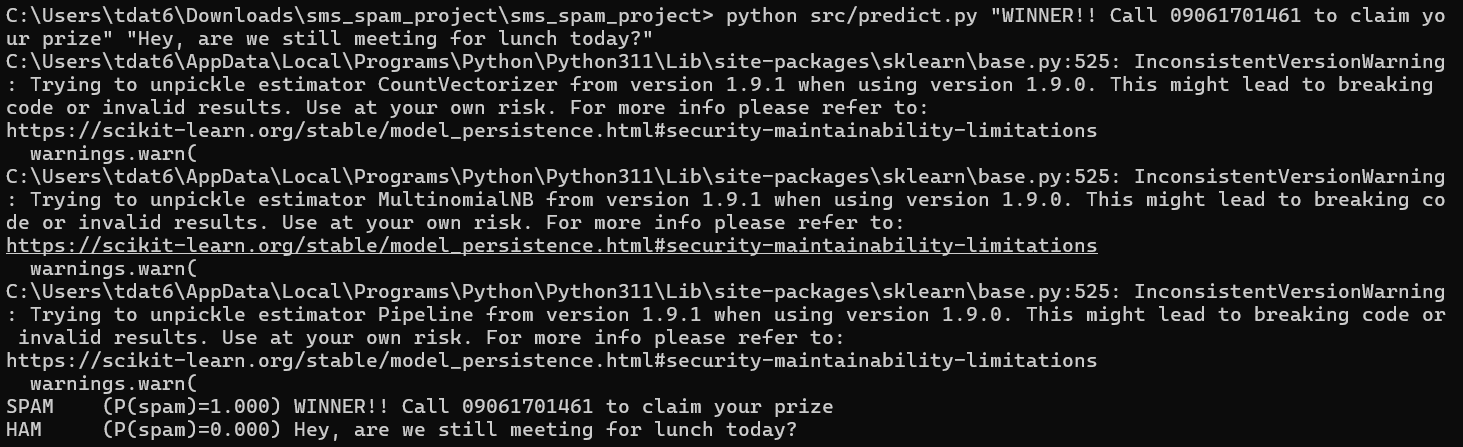
\includegraphics[width=0.95\textwidth]{images/demo_cli_predict.png}
        \caption{Minh chứng thực thi công cụ dòng lệnh CLI src/predict.py trong Terminal}
        \label{fig:demo-cli-predict}
    \end{figure}
    \begin{lstlisting}[language=bash]
python src/predict.py "WINNER!! Call 09061701461 to claim your prize" "Hey, are we still meeting for lunch today?"
    \end{lstlisting}
    Chương trình lập tức trả về kết quả chuẩn hóa dạng tab-separated:
    \begin{lstlisting}[language=bash]
SPAM    (P(spam)=1.000)    WINNER!! Call 09061701461 to claim your prize
HAM     (P(spam)=0.000)    Hey, are we still meeting for lunch today?
    \end{lstlisting}
    
    \item \textbf{Chế độ tương tác nhập liệu liên tục (Interactive shell):}
    Khi chạy lệnh \texttt{python src/predict.py} không kèm đối số, chương trình mở một dấu nhắc lệnh tương tác \texttt{$>$ }, cho phép người dùng gõ liên tục từng tin nhắn và nhận kết quả tức thời, kết thúc bằng một dòng trống.
\end{enumerate}

\section{Tổng kết các kết quả đạt được của đề tài}
\label{sec:tong-ket-ket-qua}

Sau quá trình nghiên cứu lý thuyết, thiết kế hệ thống, thực nghiệm quy mô lớn và phát triển ứng dụng, Nhóm 13 đã hoàn thành xuất sắc toàn bộ các mục tiêu đặt ra với những kết quả nổi bật:
\begin{enumerate}
    \item \textbf{Xây dựng quy trình học máy NLP hoàn chỉnh và chuẩn mực:} Hoàn thiện chu trình khép kín từ tiền xử lý dữ liệu thô, loại bỏ 403 mẫu trùng lặp, chia tách Stratified Train/Test 80/20, đóng gói đường ống \texttt{Pipeline} kiểm soát 100\% nguy cơ rò rỉ dữ liệu (Data Leakage).
    \item \textbf{Sáng tạo kỹ thuật tiền xử lý bảo toàn tín hiệu cấu trúc:} Kỹ thuật quy đổi số dài, URL, tiền tệ thành các token đặc biệt (\texttt{longnumtoken}, \texttt{urltoken}, \texttt{currtoken}) đã chứng minh hiệu quả vượt bậc, đóng góp tới $74,6\%$ tầm quan trọng của Cây quyết định và cải thiện rõ rệt điểm F1 của toàn bộ hệ thống.
    \item \textbf{Thực hiện khối lượng thực nghiệm đồ sộ có tính kiểm soát cao:} Khảo sát toàn diện 36 cấu hình dữ liệu ở Giai đoạn 1; thực hiện tinh chỉnh tối ưu siêu tham số chuyên sâu bằng \texttt{GridSearchCV} 5-fold CV ở Giai đoạn 2; khảo sát mở rộng độ nhạy tham số $\alpha \in [0.1, 10.0]$; phân tích độc lập tác động của n-gram, \texttt{min\_df}, \texttt{max\_df} và giới hạn \texttt{max\_features}.
    \item \textbf{Khẳng định mô hình tối ưu toàn diện:} Xác lập \textbf{Multinomial Naive Bayes} ($\alpha=2.0$, P2, BoW unigram) là mô hình dẫn đầu với F1-score kiểm thử đạt \textbf{$0,9653$}, Recall \textbf{$95,42\%$}, Accuracy \textbf{$99,13\%$}, tốc độ dự đoán cực nhanh $27.900$ tin/giây và duy trì độ ổn định cao nhất qua 5 seed ngẫu nhiên ($F_1 = 0,9467 \pm 0,0195$).
    \item \textbf{Khám phá các phát hiện khoa học và cạm bẫy dữ liệu sâu sắc:} Chỉ ra sai lầm phương pháp luận khi đánh giá TF-IDF trên tham số mặc định $\alpha=1.0$; giải thích thất bại của khoảng cách Euclid trên K-NN; vạch trần cạm bẫy dữ liệu HTML \texttt{lt}/\texttt{gt} sinh ra từ quá trình ẩn danh hóa số điện thoại.
    \item \textbf{Phát triển ứng dụng Demo và CLI hoàn thiện:} Xây dựng thành công ứng dụng web Streamlit trực quan, hỗ trợ so sánh đa mô hình, bộ 8 kịch bản kiểm thử mẫu và cơ chế giải thích quyết định XAI minh bạch.
\end{enumerate}

\section{Hướng nghiên cứu và phát triển mở rộng trong tương lai}
\label{sec:huong-phat-trien}

Mặc dù hệ thống đã đạt được hiệu năng rất cao trên bộ ngữ liệu thực nghiệm, để tiến tới triển khai một giải pháp lọc tin nhắn thương mại thực thụ trong môi trường viễn thông thực tế, nhóm đề xuất một số hướng nghiên cứu và phát triển mở rộng:
\begin{enumerate}
    \item \textbf{Tối ưu hóa ngưỡng cắt quyết định (Decision Threshold Tuning):}
    Trong hệ thống hiện tại, ngưỡng phân loại xác suất mặc định là $\tau = 0.5$. Trong môi trường vận hành thực tế nơi chi phí của lỗi Dương tính giả (FP) là cực kỳ đắt, có thể dịch chuyển ngưỡng quyết định lên mức khắt khe hơn (ví dụ $\tau = 0.8$ hoặc $\tau = 0.9$) hoặc tối ưu hóa ngưỡng dựa trên đường cong Precision-Recall nhằm triệt tiêu hoàn toàn nguy cơ chặn nhầm tin nhắn quan trọng của khách hàng.
    \item \textbf{Mở rộng ngữ liệu và thích ứng đa ngôn ngữ (Tiếng Việt):}
    Thu thập và gán nhãn tập ngữ liệu tin nhắn rác tiếng Việt hiện đại, tích hợp các công cụ tách từ tiếng Việt chuyên biệt (như \texttt{pyvi}, \texttt{underthesea}) và bổ sung các mẫu tin nhắn lừa đảo tài chính thế hệ mới (mạo danh biến động số dư ngân hàng, bẫy đầu tư tài chính, lừa đảo việc làm online).
    \item \textbf{Ứng dụng các mô hình học sâu và biểu diễn ngữ nghĩa tiên tiến (Deep Learning \& Transformers):}
    Thử nghiệm các kiến trúc n-gram ký tự (Character-level n-grams) để chống lại thủ đoạn cố tình viết sai chính tả (ví dụ: *“cl4im pr1ze”*), kết hợp các mô hình ngôn ngữ tiền huấn luyện tiên tiến (như BERT, RoBERTa hoặc PhoBERT cho tiếng Việt) để nắm bắt sâu sắc ngữ cảnh toàn cục của câu văn.
    \item \textbf{Đóng gói vi dịch vụ (Microservices Containerization) và Triển khai Đám mây:}
    Đóng gói toàn bộ hệ thống phân loại thành các Docker container chuẩn hóa, xây dựng giao diện lập trình ứng dụng RESTful API bằng FastAPI, và tích hợp cơ chế lắng nghe phản hồi của người dùng (User Feedback Loop) để liên tục tái huấn luyện mô hình (Online Active Learning).
\end{enumerate}

\section{Tóm tắt chương 6}
Chương 6 đã khép lại công trình nghiên cứu bằng việc giới thiệu trọn vẹn sản phẩm ứng dụng demo tương tác Streamlit và công cụ dòng lệnh CLI. Hệ thống cung cấp khả năng phân loại tức thời, đối sánh đa mô hình trực quan và giải thích quyết định dựa trên đóng góp log-odds của từng từ vựng. Bộ 8 kịch bản kiểm thử mẫu được thiết kế công phu đã làm nổi bật các sắc thái kỹ thuật đa dạng giữa ba trường phái học máy. Chương này cũng đã tổng kết toàn diện các đóng góp nổi bật của đề tài và vạch ra lộ trình phát triển rõ ràng để nâng cấp hệ thống thành một giải pháp an ninh viễn thông thương mại vững chắc.